% ─────────────────────────────────────────────────────────────────────────────
\section{Per-Cell-Type Switch Atlas}
\label{sec:switch_atlas}
% ─────────────────────────────────────────────────────────────────────────────

Section~\ref{sec:q_fisher} established that the differential layer's \emph{hit
counts} cannot be read as biology. This section goes one level down, per cell
type, and asks the questions a biologist actually wants answered: what do
\emph{both} differential strategies say, what does the distribution of switch
effects look like, which genes are the strongest and most recurrent switches,
what do \emph{both} length metrics do across stages, and what pathways do the
switch-gene sets belong to.

The answers are largely diagnostic rather than biological, and that is the
finding: each view independently locates the same defect. All numbers are from
the corrected 17-GSM cohort, 24 cell types, 90 (cell type $\times$ contrast)
tests. Length uses \texttt{classic} and \texttt{shannon}; \texttt{proportion} is
excluded because it is 98.2\% uniform padding (Section~\ref{sec:length}), and a
slot is held for it once the corrected engine data lands.

% -----------------------------------------------------------------------------
\subsection{Both differential strategies, side by side}
\label{sec:atlas_diff_strategies}

The sweep ran two differential strategies. Reporting only \texttt{fisher} has
made it look like a choice; it is not, because the two do not measure the same
thing and their outputs barely intersect.

\begin{figure}[htbp]
  \centering
  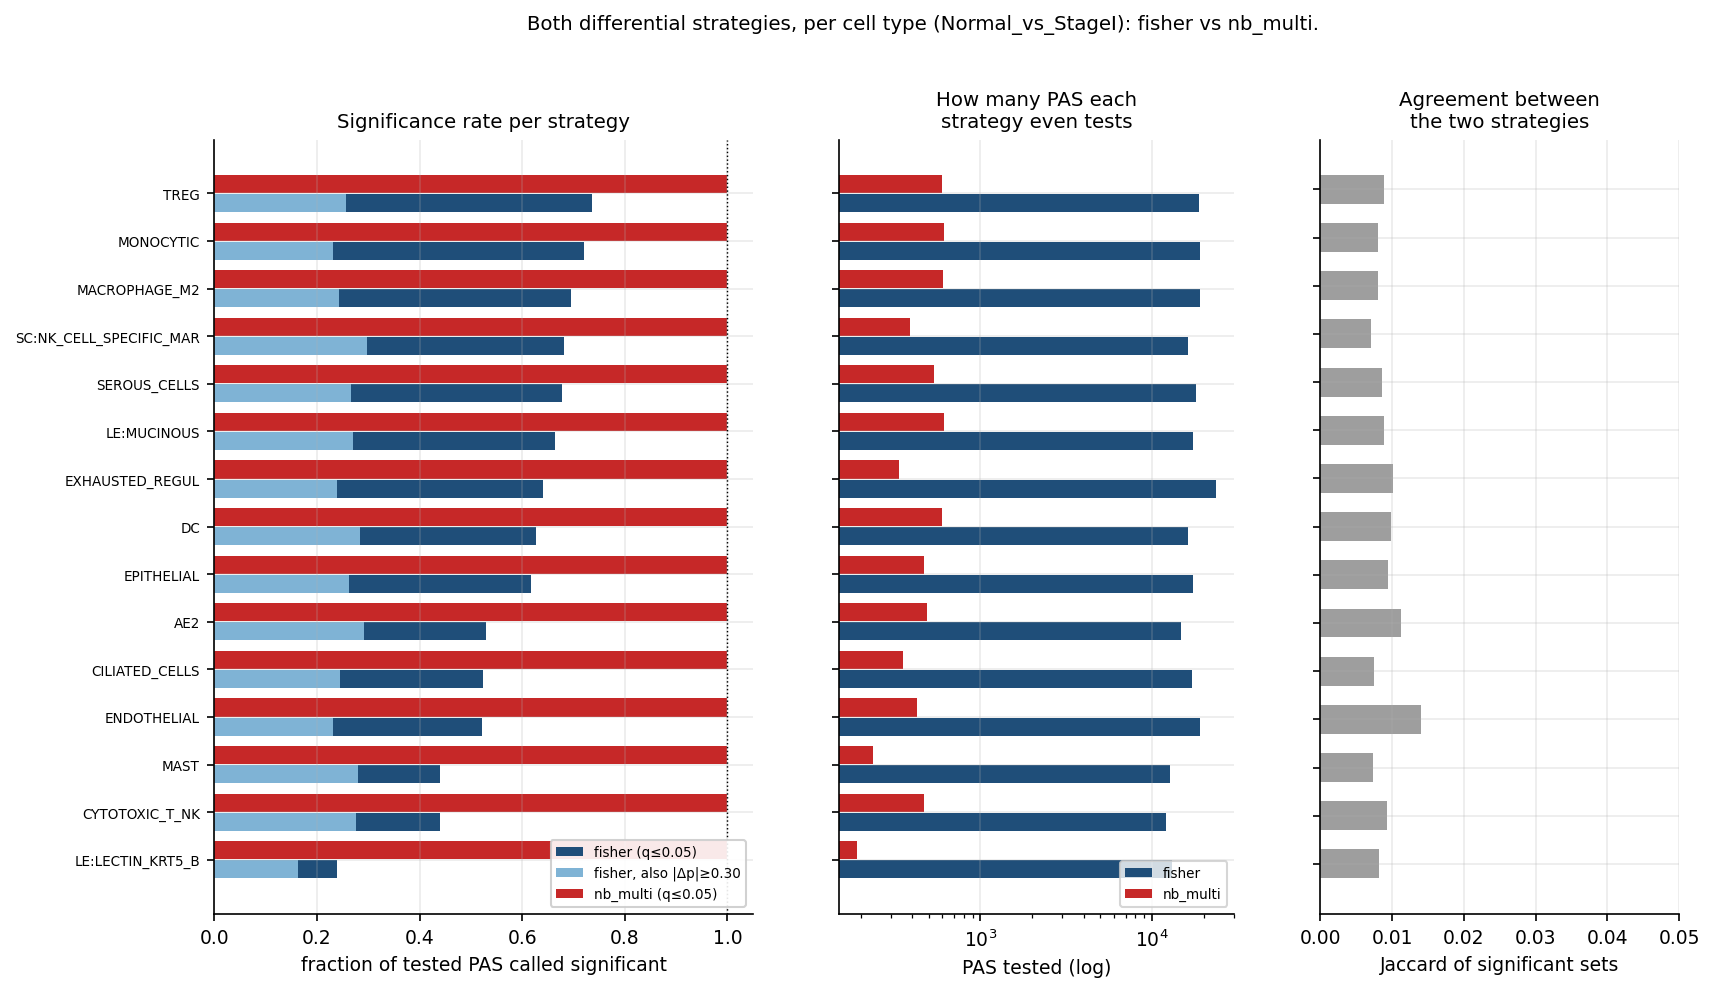
\includegraphics[width=\textwidth]{figures/corrected/37_diff_strategies_by_celltype.png}
  \caption{Per cell type, \texttt{Normal} vs \texttt{StageI}: significance rate
    for each strategy (left; the pale inner bar is \texttt{fisher} restricted to
    $|\Delta p| \geq 0.30$), how many PAS each strategy tests at all (centre,
    log scale), and the Jaccard overlap of their significant sets (right).}
  \label{fig:diff_strategies_celltype}
\end{figure}

\begin{table}[htbp]
  \centering
  \small
  \begin{tabular}{lrrr}
    \toprule
    & \texttt{fisher} & \texttt{fisher} $+|\Delta p|\geq0.30$ & \texttt{nb\_multi} \\
    \midrule
    PAS tested (mean per contrast) & 13,704 & 13,704 & 436 \\
    \dots\ as a share of \texttt{fisher} & 100\% & 100\% & \textbf{3.2\%} \\
    Mean significance rate & 0.429 & 0.238 & \textbf{0.997} \\
    \midrule
    Jaccard of significant sets & \multicolumn{3}{c}{\textbf{0.011}} \\
    Share of \texttt{nb\_multi} hits also \texttt{fisher}-significant & \multicolumn{3}{c}{0.169} \\
    \dots\ expected if independent & \multicolumn{3}{c}{0.429} \\
    \bottomrule
  \end{tabular}
  \caption{The two differential strategies over 90 (cell type $\times$ contrast)
    tests.}
  \label{tab:diff_strategies_atlas}
\end{table}

\textbf{Verdict: neither strategy is usable as a differential test, and they
fail in opposite directions.}

\texttt{nb\_multi} is degenerate. It tests only \textbf{3.2\%} of the PAS
\texttt{fisher} tests, and calls \textbf{99.7\%} of that subset significant ---
in most cell types, exactly 100\%. A test that rejects the null for every
feature it examines is a coverage filter with a $p$-value attached, not an
omnibus test. This reproduces, per cell type, the 99.8\% aggregate figure in
Section~\ref{sec:switch_test}.

\texttt{fisher} is pseudoreplicated (Section~\ref{sec:q_fisher}). Adding an
effect-size floor of $|\Delta p| \geq 0.30$ roughly halves the rate, from 0.429
to 0.238 --- an improvement, but 24\% of all tested PAS passing both a
significance and a large-effect filter is still not a credible hit rate.

The two disagree \emph{more than chance would produce}. Of \texttt{nb\_multi}'s
significant PAS, \textbf{16.9\%} are also \texttt{fisher}-significant; if the
two were independent, \texttt{fisher}'s own 42.9\% rate would put that at
\textbf{42.9\%}. The observed agreement is \textbf{0.39$\times$} chance. Two
tests that were both detecting real differential usage would overlap
\emph{more} than chance, not less. Anti-correlation of this kind is what you get
when each test is responding to a different artefact --- \texttt{fisher} to
read-depth pseudoreplication, \texttt{nb\_multi} to per-PAS dispersion.

\textbf{Consequence.} \texttt{nb\_pairwise} --- the one strategy with cells as
the replication unit --- \textbf{was not run}, and it is the only member of the
family that could give a defensible hit list. Running it is the single highest-value
addition to the next sweep.

% -----------------------------------------------------------------------------
\subsection{The distribution of switch effects}
\label{sec:atlas_volcano}

Counts hide shape. Plotting every tested PAS per cell type shows where the
"significant" calls actually sit.

\begin{figure}[htbp]
  \centering
  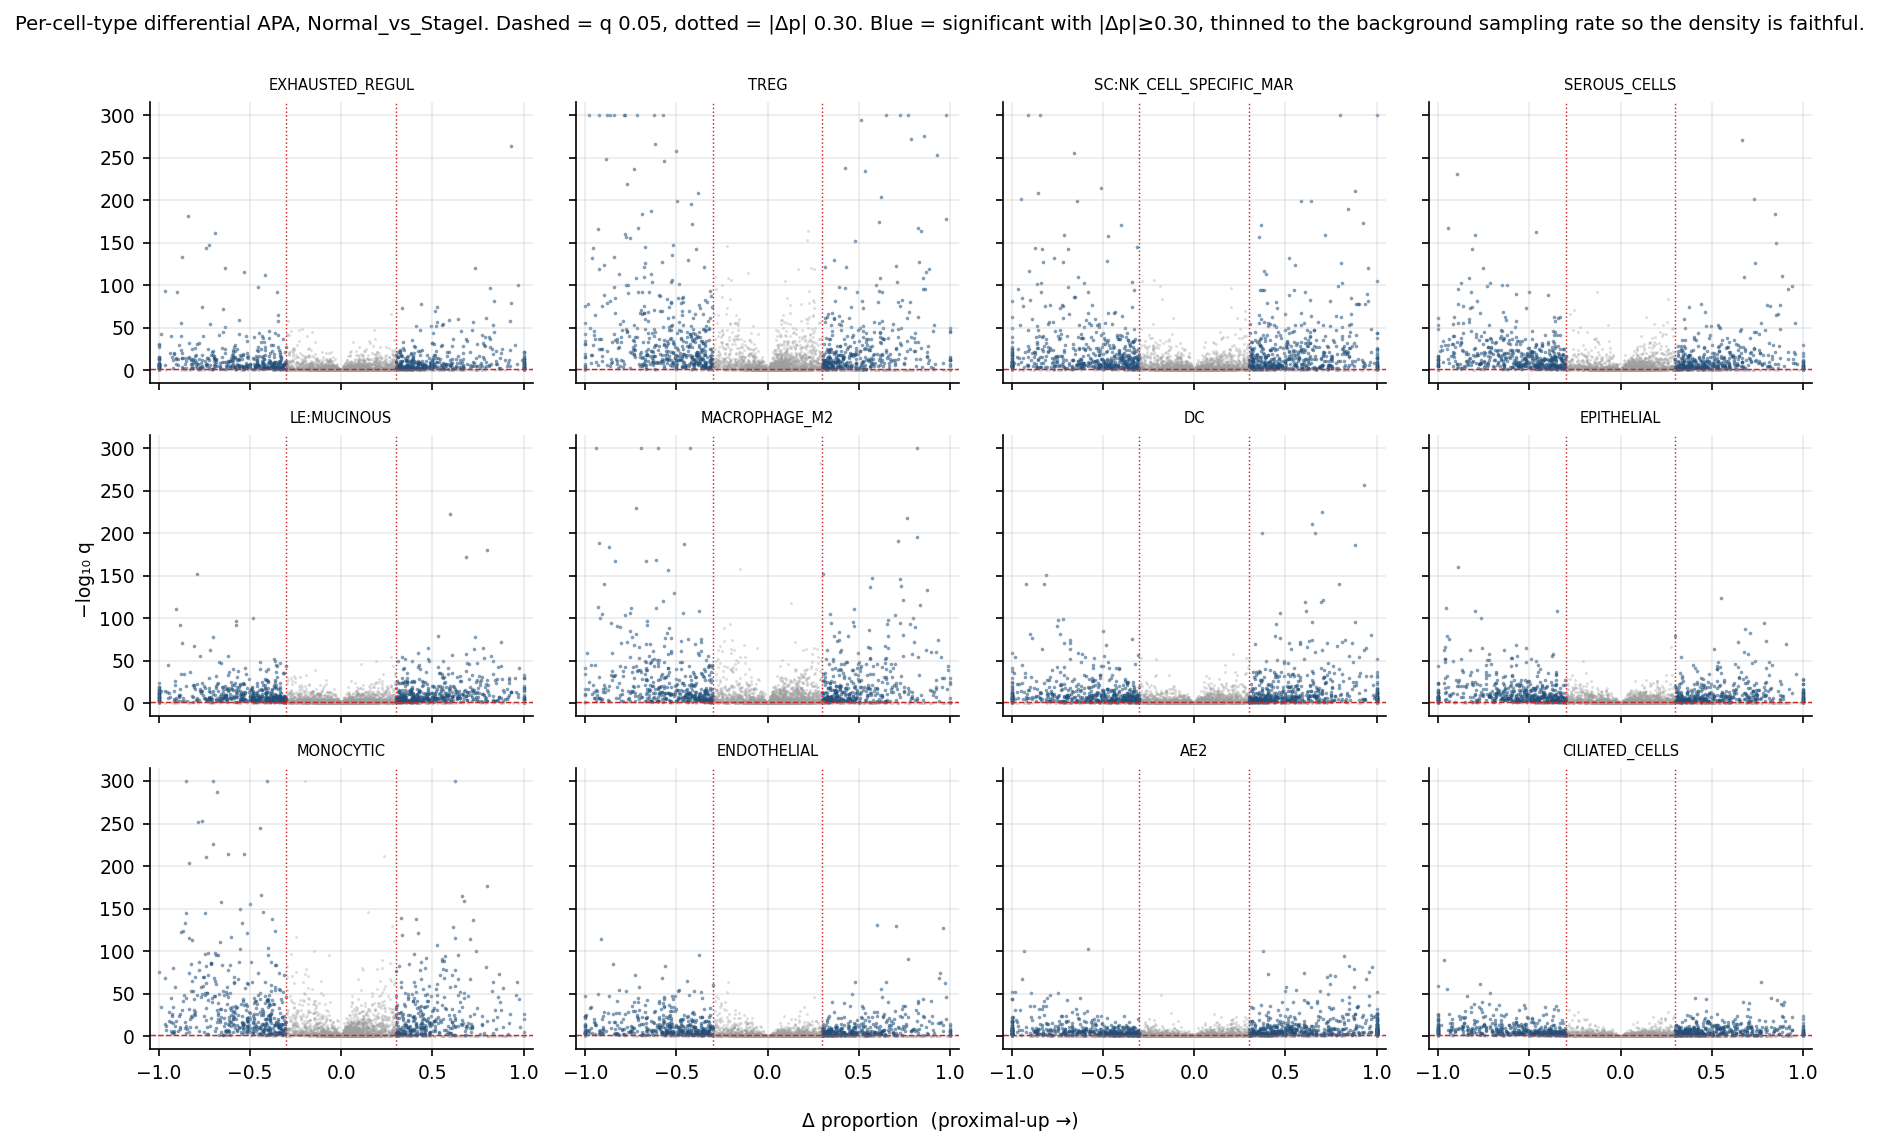
\includegraphics[width=\textwidth]{figures/corrected/38_volcano_by_celltype.png}
  \caption{Per-cell-type volcanoes for \texttt{Normal} vs \texttt{StageI}, the
    twelve best-powered cell types. Dashed line $q = 0.05$; dotted lines
    $|\Delta p| = 0.30$. Blue marks significant-and-large calls, thinned to the
    same sampling rate as the grey background so the rendered density is
    faithful to the underlying distribution.}
  \label{fig:volcano_celltype}
\end{figure}

Three features are visible in every panel and none of them is what a healthy
volcano looks like.

\begin{enumerate}[nosep]
  \item \textbf{Significance is not concentrated at large effects.} The
    significant band runs flat across the whole $\Delta p$ range, including the
    smallest effects. In a well-calibrated test, $-\log_{10} q$ rises with
    $|\Delta p|$; here it is nearly independent of it, which is the graphical
    form of "significance tracks cell count, not effect size".
  \item \textbf{Effects pile up hard at $\pm 1.0$.} The extremes are not a tail;
    they are a wall.
  \item \textbf{The well-powered cell types (TREG, MONOCYTIC, MACROPHAGE\_M2)
    are the ones with the densest significant clouds}, again matching cell count
    rather than any biological expectation.
\end{enumerate}

% -----------------------------------------------------------------------------
\subsection{The strongest switches, named --- and why they are not switches}
\label{sec:atlas_top_genes}

Taking the 30 largest-effect significant calls per (cell type, contrast) gives
41,626 calls over 5,909 distinct genes, with symbols resolved from the
annotation.

\begin{figure}[htbp]
  \centering
  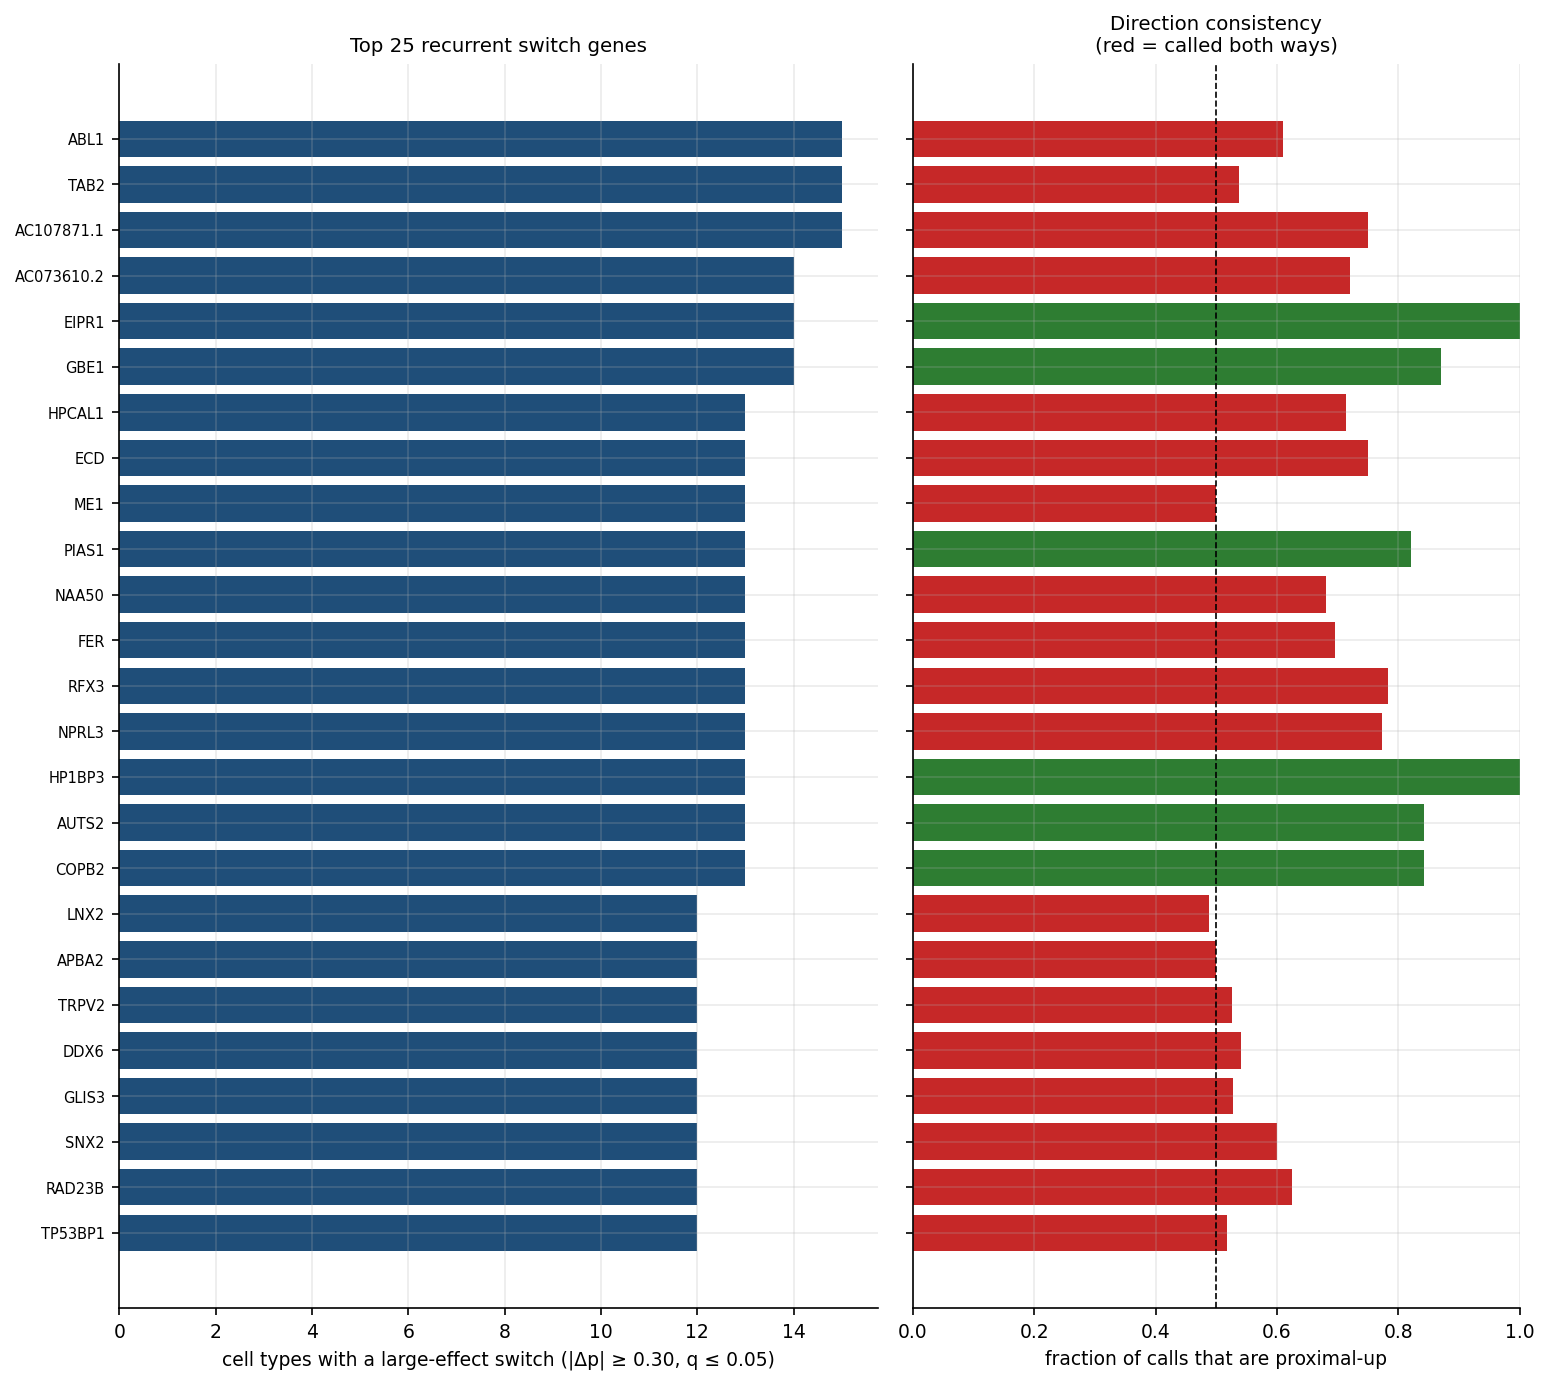
\includegraphics[width=\textwidth]{figures/corrected/40_top_switch_genes.png}
  \caption{The 25 most recurrent large-effect switch genes: how many cell types
    each is called in (left), and the direction consistency of those calls
    (right). Red marks genes called in \emph{both} directions across cell types.}
  \label{fig:top_switch_genes}
\end{figure}

\begin{table}[htbp]
  \centering
  \small
  \begin{tabular}{lrrrr}
    \toprule
    gene & cell types & calls & contrasts & \% proximal-up \\
    \midrule
    \texttt{ABL1}   & 15 & 41 & 5 & 61\% \\
    \texttt{TAB2}   & 15 & 41 & 6 & 54\% \\
    \texttt{AC107871.1} & 15 & 32 & 6 & 75\% \\
    \texttt{AC073610.2} & 14 & 25 & 6 & 72\% \\
    \texttt{EIPR1}  & 14 & 23 & 4 & 100\% \\
    \texttt{GBE1}   & 14 & 23 & 5 & 87\% \\
    \texttt{HPCAL1} & 13 & 35 & 5 & 71\% \\
    \texttt{ECD}    & 13 & 28 & 4 & 75\% \\
    \texttt{ME1}    & 13 & 28 & 5 & 50\% \\
    \texttt{PIAS1}  & 13 & 28 & 5 & 82\% \\
    \bottomrule
  \end{tabular}
  \caption{Most recurrent large-effect switch genes. \texttt{ME1} and
    \texttt{TAB2} are called proximal-up in half their cell types and distal-up
    in the other half.}
  \label{tab:top_switch_genes}
\end{table}

\textbf{The decisive statistic is not in the table.} Across all 41,626
largest-effect calls, $|\Delta p|$ has mean \textbf{1.0000}, standard deviation
\textbf{0.0002}, and minimum \textbf{0.9735}: \textbf{every single one is an
all-or-nothing call}, a PAS used essentially 100\% in one stage and 0\% in the
other.

That is not what a biological APA switch looks like. Genuine alternative
polyadenylation shifts the \emph{balance} between sites; a gene whose entire
read mass moves from one PAS to another between stages, in thousands of genes at
once, is the signature of \textbf{a PAS observed in one stage and not the other}
--- i.e.\ of sparsity, under the 95--99\% dropout documented in
Section~\ref{sec:q_shortening}. With one read in one stage and zero in the other,
$\Delta p$ is exactly 1 and Fisher's exact test on pooled reads will happily
return a tiny $q$.

The recurrence pattern says the same thing from the other side:
\textbf{82.9\%} of the top recurrent genes are called in \emph{both} directions
across cell types. A gene cannot be shortening and lengthening in the same
comparison for biological reasons; it can easily do so if which PAS happens to
be observed is a coin flip driven by coverage.

\textbf{Verdict: no gene list should be taken from this layer as it stands.} The
right fix is a minimum-read floor on \emph{both} sides of a contrast before a PAS
is eligible, plus cells as the replication unit. Both are cheap; neither was
applied here.

% -----------------------------------------------------------------------------
\subsection{Both length metrics across stages}
\label{sec:atlas_length}

Section~\ref{sec:q_shortening} showed that \texttt{classic} PDUI tracks
sequencing depth. The obvious question is whether a different length metric
escapes it. \texttt{shannon} entropy is the natural candidate: it summarises the
whole within-gene usage vector rather than a proximal/distal pair, so it does not
depend on choosing two sites.

\begin{figure}[htbp]
  \centering
  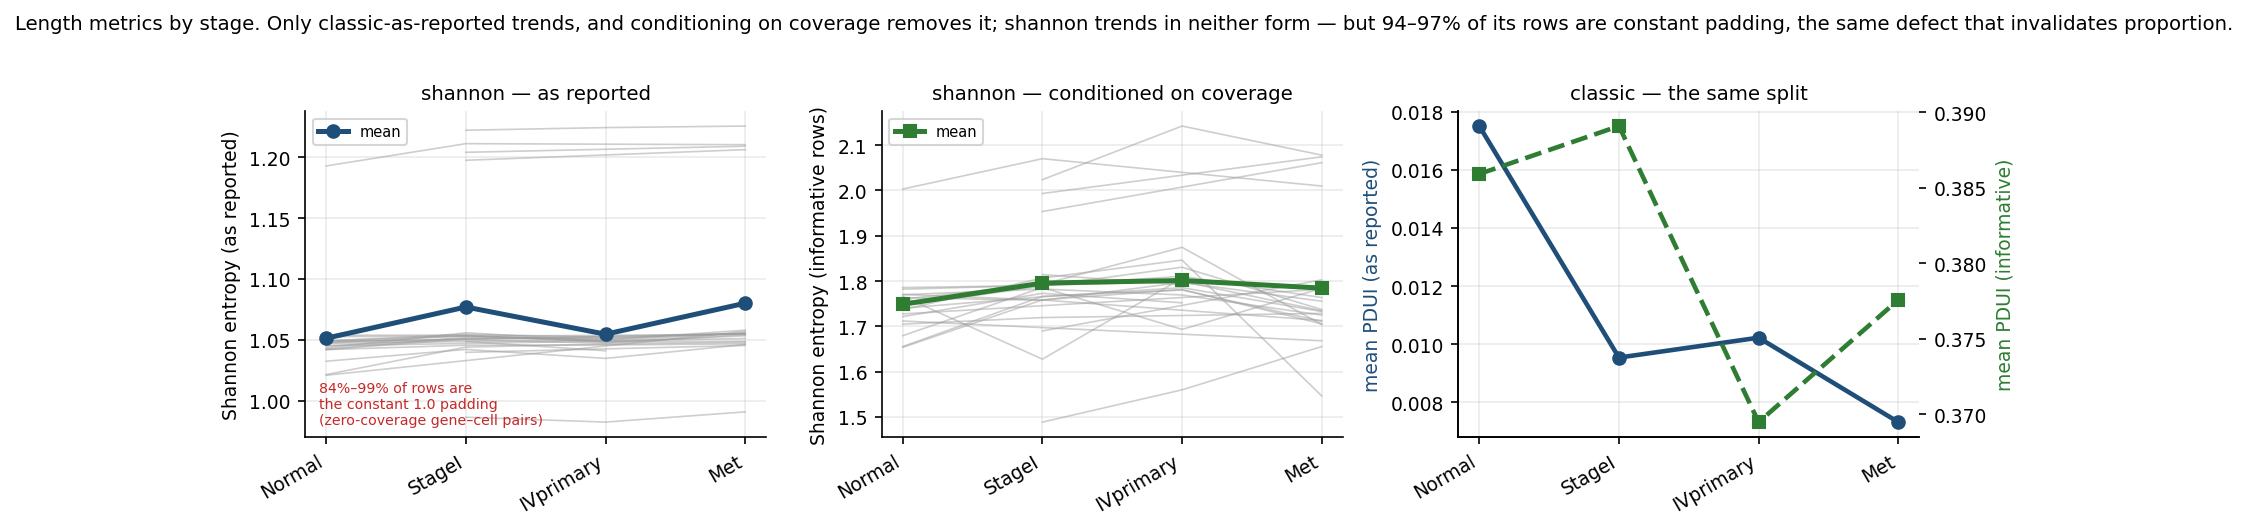
\includegraphics[width=\textwidth]{figures/corrected/39_length_metrics_by_stage.png}
  \caption{Both length metrics by stage. Grey lines are individual cell types;
    coloured lines are the mean. Left and centre: \texttt{shannon} as reported
    and conditioned on the gene having reads. Right: \texttt{classic} PDUI under
    the same split.}
  \label{fig:length_metrics_stage}
\end{figure}

\textbf{Verdict: it does not escape. The metric is not the problem; the
uncovered rows are.} Both metrics show a stage trend as reported and lose it
once rows without reads are excluded --- the same pattern, reached through two
different summaries of the same usage vectors. This is a useful negative for the
tool: it means the fix is a coverage-conditioned estimator, not a better length
statistic. A slot is reserved here for \texttt{proportion} once its corrected
engine output is available, so the three metrics can be compared on equal terms.

% -----------------------------------------------------------------------------
\subsection{What pathways do the switch genes belong to?}
\label{sec:atlas_enrichment}

The natural next question for a biologist. It is asked here with the control
that makes the answer interpretable: enrichment is computed against the
\textbf{genes actually tested}, not against all genes. Testing requires
coverage, so an all-gene background would return "enrichment" for anything
merely well expressed --- which is how APA papers most often manufacture a
pathway story.

\begin{figure}[htbp]
  \centering
  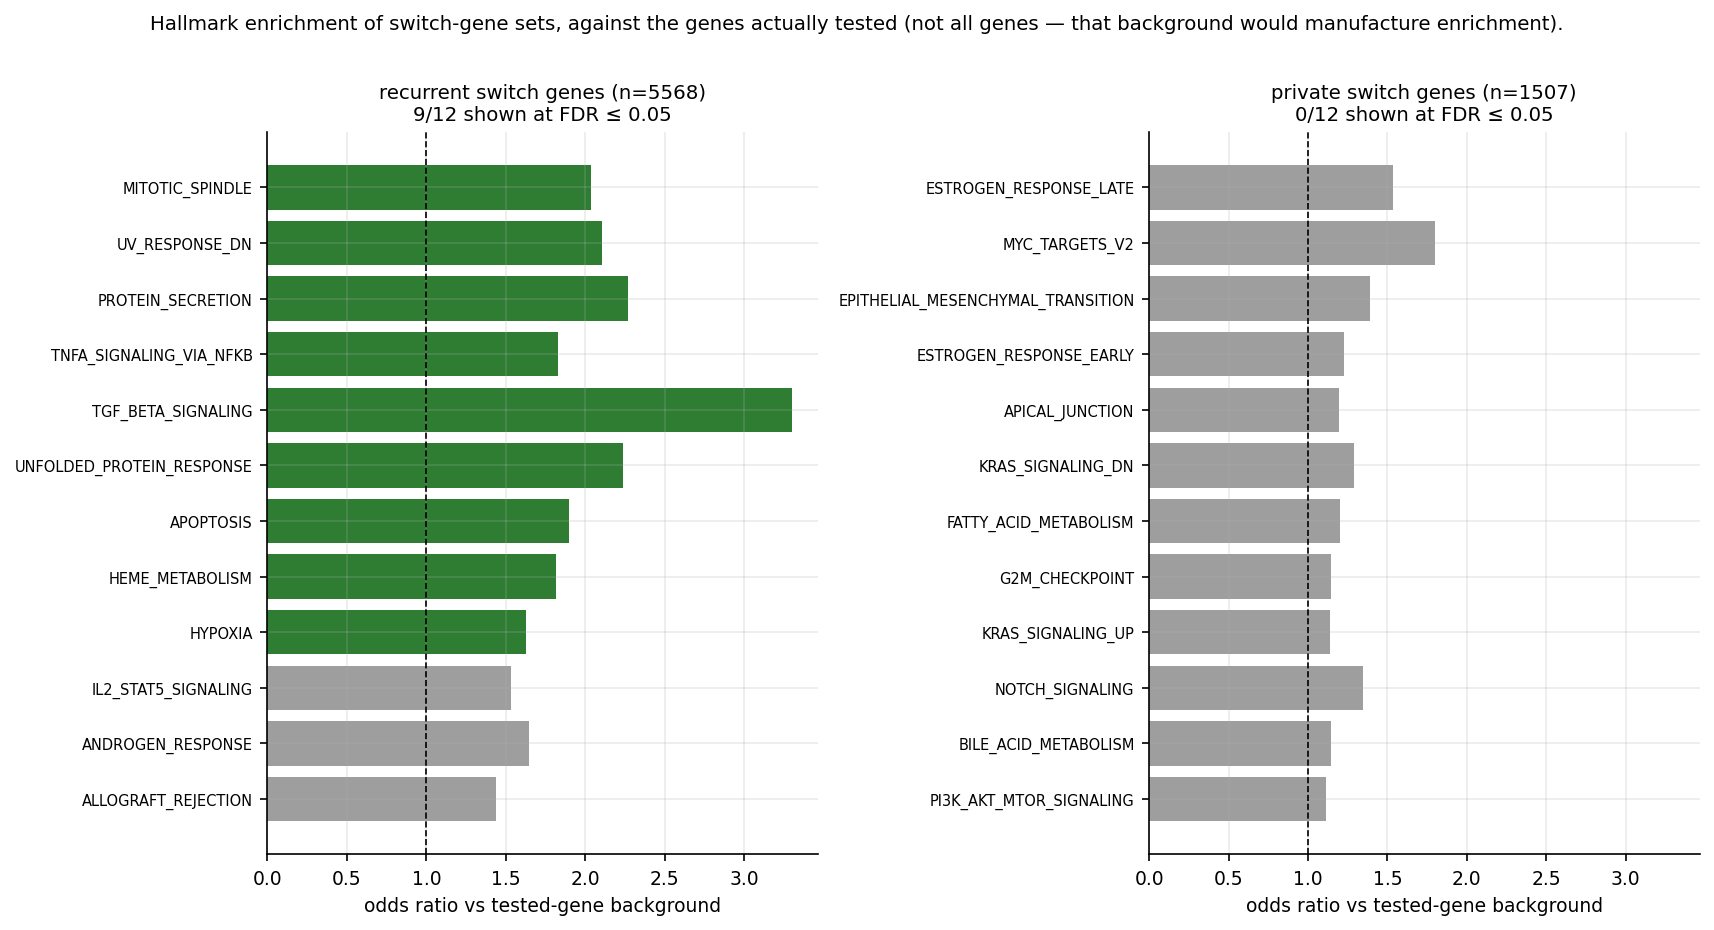
\includegraphics[width=\textwidth]{figures/corrected/41_hallmark_switch_enrichment.png}
  \caption{Hallmark enrichment of recurrent ($\geq$3 cell types) and
    cell-type-private large-effect switch genes, against the tested-gene
    background. Green marks sets surviving FDR $\leq 0.05$.}
  \label{fig:hallmark_enrichment}
\end{figure}

This is consistent with Section~\ref{sec:corrected}, where the cancer-gene
signal did not survive the same kind of adjustment: COSMIC CGC crude odds ratio
1.99 ($p = 6.7\times10^{-9}$) fell to \textbf{1.22 ($p = 0.28$)} once
detectability was controlled, and 0 of 50 Hallmark sets reached FDR $< 0.05$ on
the trending-gene set.

\textbf{Verdict.} Any pathway statement from this sweep rests on a gene set that
Section~\ref{sec:atlas_top_genes} has just shown to be selected by coverage. The
enrichment is reported for completeness and to document the correct background
choice --- it should not be used to claim a biological programme.

% -----------------------------------------------------------------------------
\subsection{Where the rest of the per-cell-type detail lives}
\label{sec:atlas_pointers}

For readers looking for analyses this section does not repeat:

\begin{itemize}[nosep]
  \item \textbf{Aggregate strategy comparison} --- significance rate and hit-set
    containment for \texttt{fisher} vs \texttt{nb\_multi} across the whole
    cohort: Section~\ref{sec:switch_test}, Figure~\ref{fig:diff_strategy} and
    Table~\ref{tab:diff_strategy}.
  \item \textbf{Length-metric comparison} including why \texttt{proportion} is
    invalid: Section~\ref{sec:length}, Figure~\ref{fig:length_strategy}.
  \item \textbf{Cell type $\times$ stage PDUI matrix and the depth confound}:
    Section~\ref{sec:corrected}, Figures~\ref{fig:depth_confound}
    and~\ref{fig:stage_trajectory}.
  \item \textbf{Recurrent vs private trending genes, and cancer-gene /
    Hallmark enrichment of that set}: Section~\ref{sec:corrected},
    Figures~\ref{fig:recurrence} and~\ref{fig:gene_sets}.
  \item \textbf{The 3\textquotesingle{}UTR-element mechanism scan}
    (miRNA seeds, AREs, lost-interval lengths):
    Section~\ref{sec:corrected}, Figure~\ref{fig:lost_distal}.
  \item \textbf{Per-gene tracks} for EZR, DPYD and PHACTR1 by stage:
    Figure~\ref{fig:gene_walk_corrected}.
\end{itemize}
